\section{Methodology}
\label{sec:method}

\subsection{Experimental setup}
\label{sec:expt_setup}

To evaluate our proposal on real hardware, we implement Splitwise's KV-cache transfer mechanism on top of vLLM~\cite{vllm}. Our implementation is open source~\cite{splitwise_vllm_pr}.
We run this modified vLLM on two DGX-A100 and two DGX-H10 virtual machines (VMs) on Microsoft Azure with specifications from \Cref{tab:a100_vs_h100_specs}.
These are the VMs used to collect the characterization data in \Cref{sec:motivation}.
These machines are connected with InfiniBand and the DGX-H100s have double the bandwidth (\ie, 400 Gbps).

Since vanilla vLLM only supports continuous batching with token preemption which can lead to much higher TBT, we implement state-of-the-art mixed continuous batching~\cite{yu2022orca} as discussed earlier in \Cref{fig:batching-gantt-chart}(c).

Our implementation of the Splitwise technique assigns machines either a prompt role, or a token role.
As the prompt machine generates the first token, it transfers the KV-cache to the token machine using the technique described in \Cref{sec:designkv}.
We use MSCCL++~\cite{mscclpp}, an optimized GPU-driven communication library, to implement the naive and layer-wise KV cache transfers.

\rev{
In our implementation, the prompt machine uses the zero-copy one-sided \texttt{put} primitive of MSCCL++ to send KV-cache data over InfiniBand as soon as it is ready, without requiring the token machine to issue any receive instructions.
Once we have issued a \texttt{put} for all layers, the prompt machine signals a semaphore that the token machine waits on.
The synchronization done with the help of semaphores uses the same InfiniBand connection used to send KV-cache data.
When processing a batch of prompts, each request is assigned a different semaphore since it may be routed to different token machines.
We ship the KV-caches block-by-block in vLLM.
To minimize the number of transfers, we also consider the contiguity of KV blocks as long as they use the same semaphore.
}

% We run this modified vLLM on two DGX-A100s and two DGX-H100s full-machine VMs on a public cloud provider with the specifications from \Cref{tab:a100_vs_h100_specs}.
% These are the VMs used to collect the characterization data in \Cref{sec:motivation}.
% These machines are connected with InfiniBand and the DGX-H100s has double the bandwidth (\ie, 400 Gbps).


\subsection{Simulator setup}
\label{sec:simulator}

%While the experimental setup to evaluate the Splitwise technique, for the evaluation of the cluster-level design, we would need tens of machines.
We build a simulator to explore cluster designs and evaluate Splitwise at scale.
The simulator code is open source~\cite{splitwise_sim}.

%\inigo{Chaojie has now validated the baseline, we should add some text about validation}

\begin{figure}[t]
    \centering
    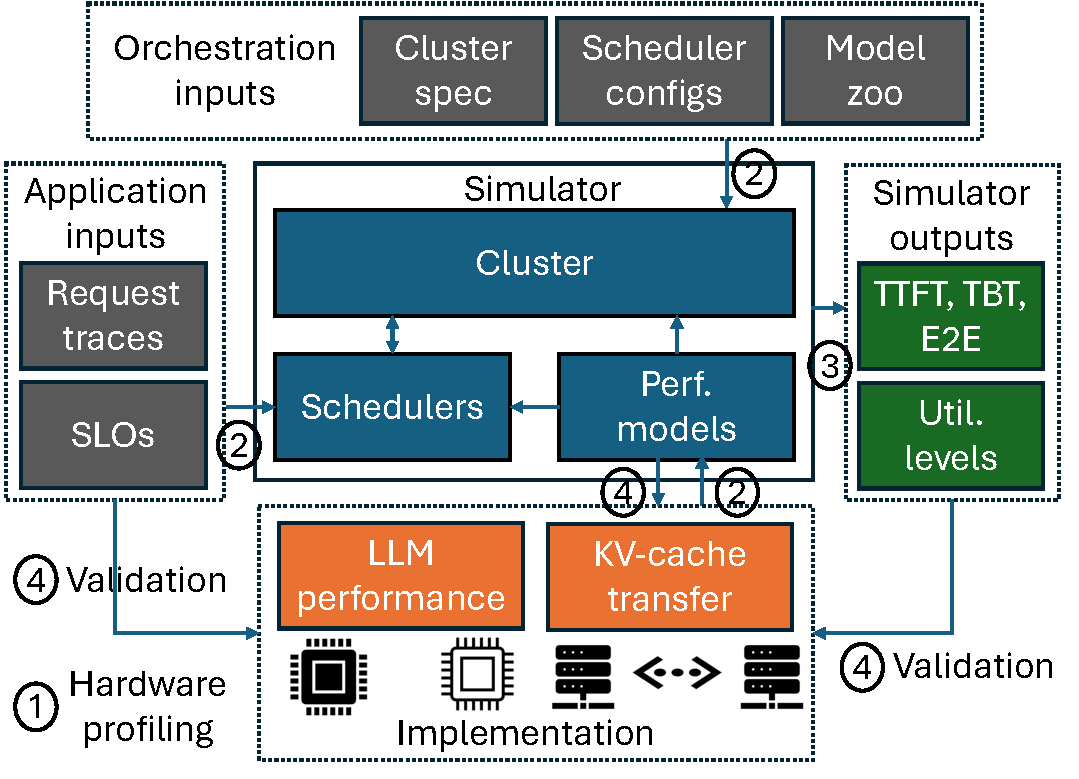
\includegraphics[width=0.75\columnwidth]{figures/splitwise_sim}
    \caption{\rev{Overview of the design of the Splitwise simulator.}}
    \label{fig:simulator}
\end{figure}

\rev{
\Cref{fig:simulator} shows the design of our simulator.
The simulator is event-driven and faithfully models the Splitwise machine pools, schedulers, machine-level memory and queues, and KV-cache transfer.
We first profile the LLM on the target hardware with various input/output sizes~\circled {1}.
Based on the characterization profiles, we build a performance model.
The simulator takes as input the request traces, SLOs, the performance model, and the configurations for cluster and scheduler~\circled {2}.
%It takes application request traces, orchestration configurations, and profiling results as inputs and provides performance metrics, approximate memory usage, and batching decisions as output. 
For our evaluation, we use the prompt and token size distributions from the production traces in \Cref{sec:motivation}.
We tune the Poisson arrival rate to increase and decrease the load (requests per second) for cluster sizing.
The simulator provides the achieved metrics per request (TTFT, TBT, E2E), and the machine utilization levels~\circled {3}.
We cross-validated the performance model with hardware experiments to ensure accuracy; we also validated the simulator end-to-end using production load with over 50K iterations to ensure fidelity~\circled {4}.
%We use TP, which provides much better performance than PP for the models we evaluate~\cite{alpaserve}. 
%The hardware profiles are used to build a performance model and a communication model, which we describe  
}


\rev{
\myparagraph{Performance model}
We build a piece-wise linear performance model using performance profiles at various batch sizes, input sizes, output sizes, in the required parallelism configuration on A100 and H100 machines from~\Cref{sec:motivation}.
%We also feed the performance impact from different prompt and token phase mixes in a batch.
We validate that our performance model has high accuracy; it incurs a mean absolute percentage error (MAPE) of less than 3\% when evaluated with a 80:20 train:test dataset split.
%\todo{Note: This validation does not include mixed batching due to few actual datapoints}
%We also use the same performance model for the entire evaluation, ensuring that requests are similarly impacted on both Splitwise and baseline systems.

\myparagraph{Communication model}
%Depending on the model parallelism and KV-cache transfer configurations, there might inter-machine and intra-machine communication.
In our evaluation, KV-cache transfers cause inter-machine communication, whereas tensor parallelism only causes intra-machine communication.
We model inter-machine communication overheads by benchmarking our KV-cache transfer implementation over Infiniband in~\Cref{sec:expresults}.
%\inigo{This previous sentence is misleading as it suggests that we are doing infiniband between A100 and H100.}
%We do not explicitly model intra-machine communication from TP, since it occurs on a separate interconnect (\ie, NVLink) and does not impact inter-machine KV-cache transfers. 
%The performance implications from TP are captured by our performance model.
}

\myparagraph{SLOs}
To determine the maximum throughput that can be supported by a given cluster design, we use P50, P90, and P99 SLOs for TTFT, TBT, and E2E latency metrics.
\Cref{tab:eval-slo} shows our SLO definition using DGX-A100 as a reference.
We require all nine SLOs to be met.
SLOs on TTFT are slightly looser, since it has a much smaller impact on the E2E latency.

\begin{table}[t]
\centering
\begin{tabular}{cccc}

\toprule
            & \textbf{P50} & \textbf{P90} & \textbf{P99} \\
     \midrule
     \textbf{TTFT}   & 2$\times$    & 3$\times$   & 6$\times$\\
     \textbf{TBT}    & 1.25$\times$ & 1.5$\times$ & 5$\times$\\
     \textbf{E2E}    & 1.25$\times$ & 1.5$\times$ & 5$\times$\\
\bottomrule
\end{tabular}
\caption{SLO expressed as slowdown compared to a request running on DGX-A100 under no contention.}
\label{tab:eval-slo}
\end{table}

\myparagraph{Baselines}
We compare our Splitwise designs against Baseline-A100 and Baseline-H100.
The clusters in these baselines consist of just DGX-A100s and DGX-H100s, respectively.
Both baselines use the same mixed continuous batching that Splitwise uses for mixed pool machines (described in \Cref{sec:scheduler}).

\section{Evaluation}
\label{sec:eval}

\subsection{Experimental results}
\label{sec:expresults}

\myparagraph{KV-cache transfer latency}
We first measure the latency to transfer the KV-cache as the prompt size grows.
\Cref{fig:kvcacheperf} shows the visible transfer latency on both A100 and H100 setups with the naive and optimized transfer design as discussed in \Cref{fig:kvcachedesign}.
Compared to the prompt computation time, the overhead is minimal ($<7\%$).
The time for serialized transfers linearly increases with the prompt size since the size of the KV-cache also increases.
The optimized per-layer transfer, on the other hand, hides much of the latency.
For these transfers, we see a constant non-overlapped transfer time of around 8ms for the A100 and around 5ms for the H100 setup.
The H100 setup has double the bandwidth of the A100 setup (\ie, 200 vs 400 Gbps), and the impact of this can be clearly seen with transfers in the H100 setup happening about twice as fast as those in the A100 setup.

As discussed in \Cref{sec:designkv}, for small prompt sizes ($<512$ in H100), Splitwise uses the serialized KV-cache transfer and for larger prompts, it uses per-layer transfers.

%\inigo{Aashaka has made optimizations and we do not need to do the serialized transfer for small prompts.}


\begin{figure}[t]
    \centering
    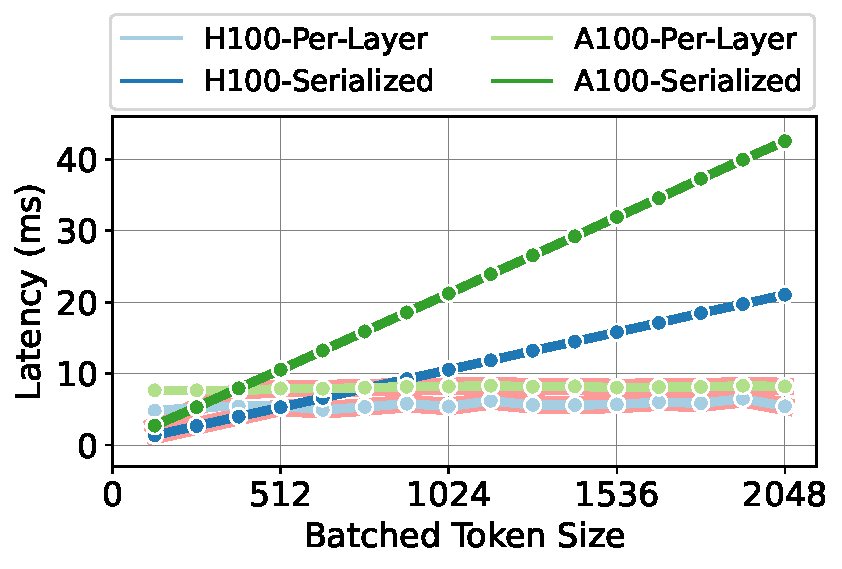
\includegraphics[width=0.6\columnwidth]{figures/eval/kv_time}
    \caption{Overhead of the KV-cache transfer as the prompt size increases on A100s and H100s.}
    \label{fig:kvcacheperf}
\end{figure}


\myparagraph{End-to-end impact}
Next, we run the coding trace on the 2-machine Splitwise setups without batching, and compare the observed latency metrics to a 1-machine baseline setup with no batching.
\Cref{fig:kvcacheperfe2e} shows our results.
The latency impact of serially transferring the KV-cache grows up to 3\% of the E2E with large prompts.
However, Splitwise only incurs 0.8\% of E2E.
In a user-facing inference, the only visible impact of KV-cache transfer overhead is the latency for the second token.
Splitwise adds a 16.5\% latency to the second token, as compared to the 64\% overhead from a serialized transfer.
Overall, the transfer impact in Splitwise is hardly perceivable even in a user-facing inference. 

\begin{figure}[t]
    \centering
    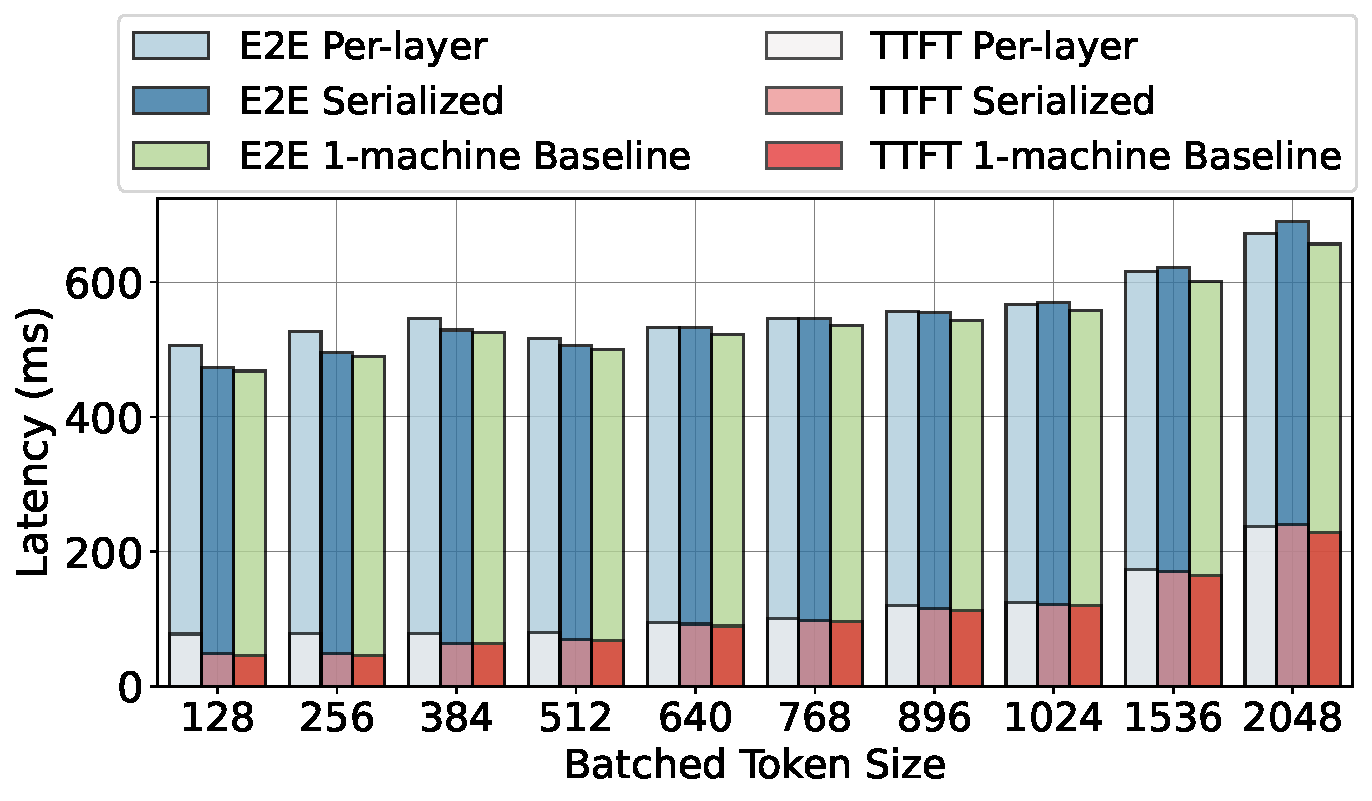
\includegraphics[width=0.7\columnwidth]{figures/eval/kv_e2e_time.pdf}
    \caption{Overhead of KV cache transfer on TTFT, E2E latency for coding trace for A100 and H100.}
    \label{fig:kvcacheperfe2e}
\end{figure}



\subsection{Iso-power throughput-optimized clusters}

\myparagraph{Cluster provisioning}
We provision clusters using the methodology described in \Cref{sec:provision}.
We target a specific workload (\eg, conversation) at a peak load with the same power (\ie, iso-power) for each cluster design.
For the baseline, we use the power for 40 DGX-H100 machines as our target peak power.
For the A100 baseline, we can fit 70 DGX-A100 machines under the same power budget.
We denote these two designs as 40P/T and 70P/T respectively, since they both use mixed batching in all machines.

For Splitwise cluster designs under the coding trace, Splitwise-AA provisions 55 prompt machines and 15 for the token pool, denoted as (55P, 15P).
Note that like Baseline-A100, Splitwise-AA also provisions 75\% more machines than Baseline-H100.
The legends in \Cref{fig:isopowerfull} show the different provisioning choices under coding and conversation workloads.
Request size distributions reflect in the machine pool sizing.
For example, we provision more prompt machines under Splitwise-HH (35P, 5T) for the coding trace, while we provision more token machines (25P, 15T) for the conversation trace.


\myparagraph{Latency and throughput}
\Cref{fig:isopowerfull} shows a deep dive into all the latency metrics at different input load for each cluster design with the same power (\ie, iso-power).
For the coding trace (\Cref{fig:isopowerfullcode}), Splitwise-HH, Splitwise-HHcap, and Splitwise-AA all perform better than Baseline-H100.
As the load increases, Baseline-H100 suffers from high TBT due to mixed batching with large prompt sizes.
Although Splitwise-AA can support higher throughput, its TTFT is consistently higher than most designs.
Splitwise-HA clearly bridges the gap by providing low TTFT and E2E at high throughput.
The mixed machine pool in Splitwise becomes useful at higher loads to use all the available hardware without fragmentation.
This benefit can be seen clearly in the P50 TBT chart for Splitwise-HA, where after 90 RPS, H100 machines jump into the mixed machine pool and help reduce TBT. 

For the conversation trace (\Cref{fig:isopowerfullconv}), Splitwise-HHcap clearly does better on all fronts, including latency.
This is because its token generation phases typically run for much longer than in the coding trace, which is beneficial for the token machines.


\begin{figure}[t]
    \centering
    \subfloat[Coding trace.]{
    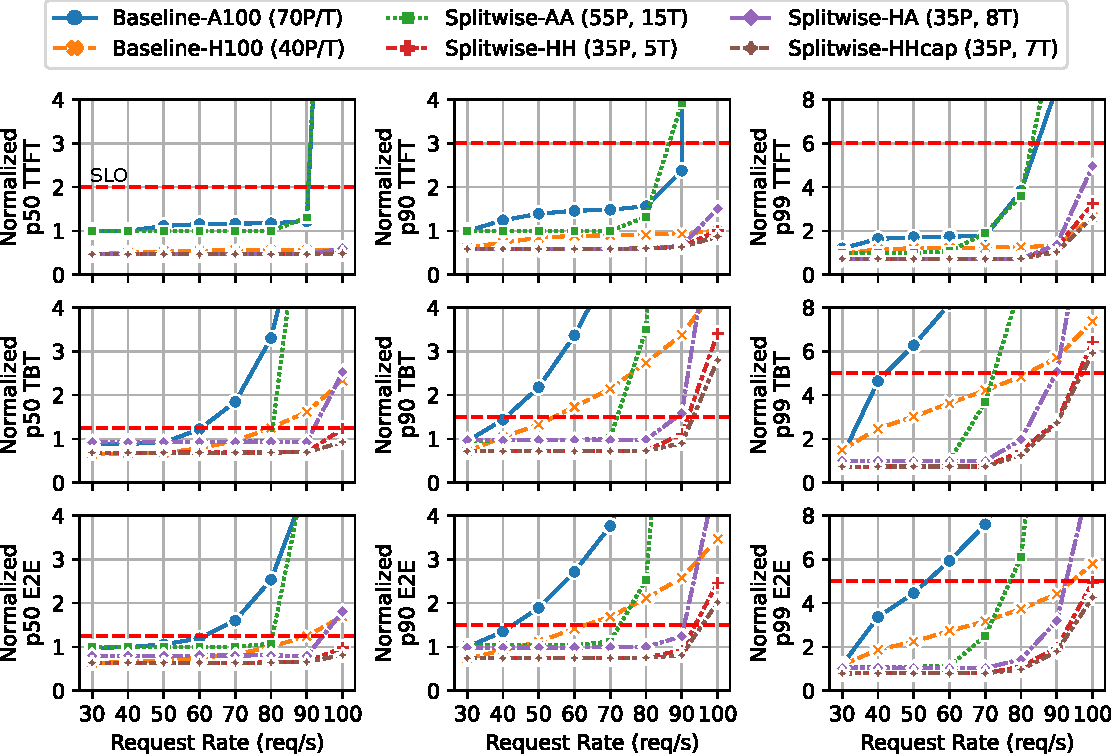
\includegraphics[width=1.0\columnwidth]{figures/eval/isopower_code_bloom-176b}
    \label{fig:isopowerfullcode}
    }
    \vspace{2pt}
    \subfloat[Conversation trace.]{
    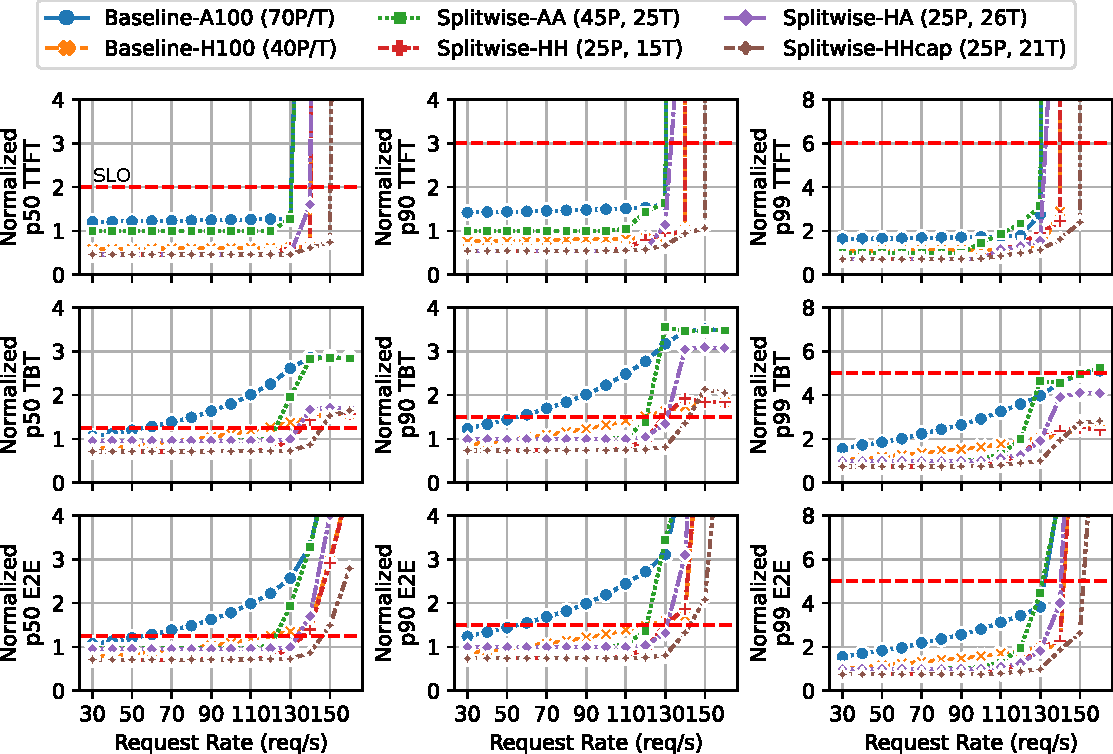
\includegraphics[width=1.0\columnwidth]{figures/eval/isopower_conv_bloom-176b}
    \label{fig:isopowerfullconv}
    }
    \caption{Latency metrics across input loads for iso-power throughput optimized clusters.
    Dashed red lines indicate SLO.
    }
    \label{fig:isopowerfull}
    %\vspace*{-0.5cm}
\end{figure}



\myparagraph{Impact on batched tokens}
\Cref{fig:batchingeval} shows the cumulative distribution of time spent processing a varying number of batched active tokens in an iso-power throughput-optimized cluster. The distributions are collected by running the conversation trace at low (70 RPS) and high (130 RPS) loads.

At low load, all 40 Baseline-H100 machines spend 70\% of the time running $\leq$15 tokens, and the rest running mixed batches with large prompts, which affects TBT and E2E.
The 35 Splitwise-HH prompt machines are mostly idle, and when active, run much larger batches of tokens.
The 15 Splitwise-HH token machines also do a better job at batching.
Overall, Splitwise machines have better batching and latency at 70 RPS.
At high load, since the mixed pool is utilized more, the batch sizes start looking similar across prompt and token machines.

\begin{figure}[t]
    \centering
     \subfloat[Low load (70 RPS).]{
        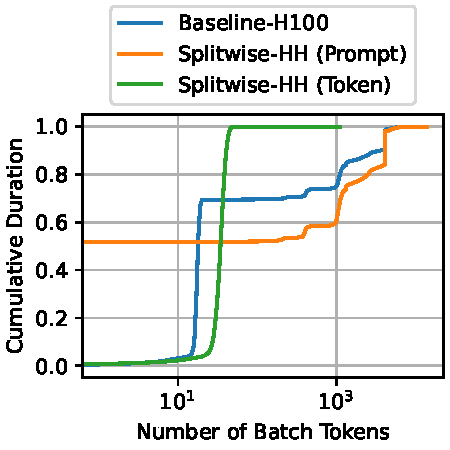
\includegraphics[width=0.48\columnwidth]{figures/eval/duration_ccdf_batch_tokens_bloom-176b_conv70.pdf}
        \label{fig:batchlowtput}
    }
    \subfloat[High load (130 RPS).]{
        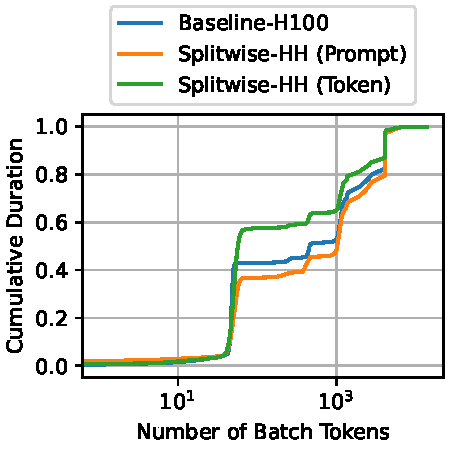
\includegraphics[width=0.48\columnwidth]{figures/eval/duration_ccdf_batch_tokens_bloom-176b_conv130.pdf}
        \label{fig:batchhightput}
    }
    \caption{Cumulative distribution of time spent at various batched token sizes for iso-power throughput-optimized design.
    }
    \label{fig:batchingeval}
\end{figure}



\myparagraph{Summary plot}
\Cref{fig:isopowertput} summarizes the results across all cluster metrics for iso-power throughput-optimized designs for the conversation trace.
We use Baseline-A100 as the baseline.
Compared to Baseline-A100, Splitwise-AA delivers 2.15$\times$ more throughput at the same power and cost.
Splitwise-HA delivers 1.18$\times$ more throughput at 10\% lower cost and the same power.

\begin{figure}[t]
    \centering
     \subfloat[Iso-power.]{
        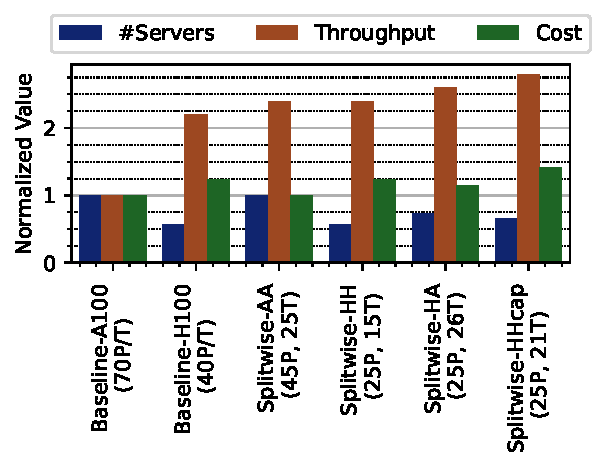
\includegraphics[width=0.48\columnwidth]{figures/eval/isopower_conv_cost_throughput_bloom-176b}
        \label{fig:isopowertput}
    }
    \subfloat[Iso-cost.]{
        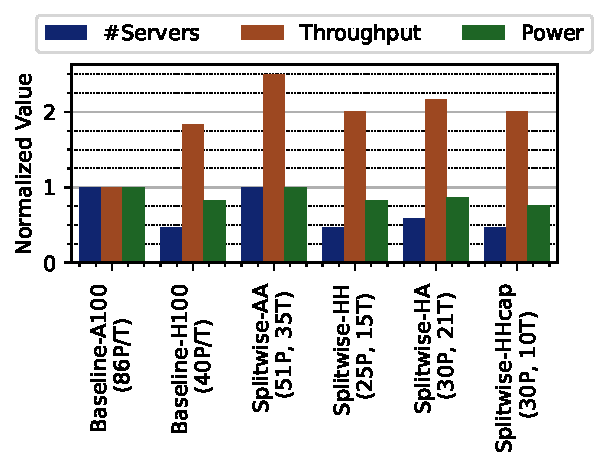
\includegraphics[width=0.48\columnwidth]{figures/eval/isocost_conv_power_throughput_bloom-176b}
        \label{fig:isocosttput}
    }
    \caption{Summary of throughput-optimized cluster designs.}
    \label{fig:throughputopt}
    \vspace*{-0.5cm}
\end{figure}


\begin{figure}[t]
    \centering
     \subfloat[Power-optimized.]{
        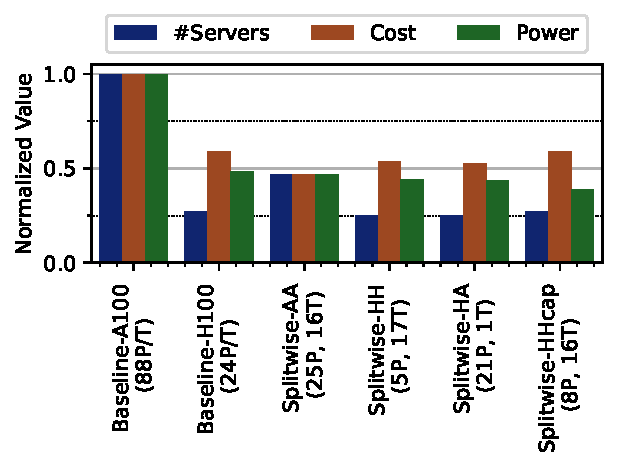
\includegraphics[width=0.48\columnwidth]{figures/eval/isothroughput_conv_power_bloom-176b}
        \label{fig:isotputpower}
    }
    \subfloat[Cost-optimized.]{
        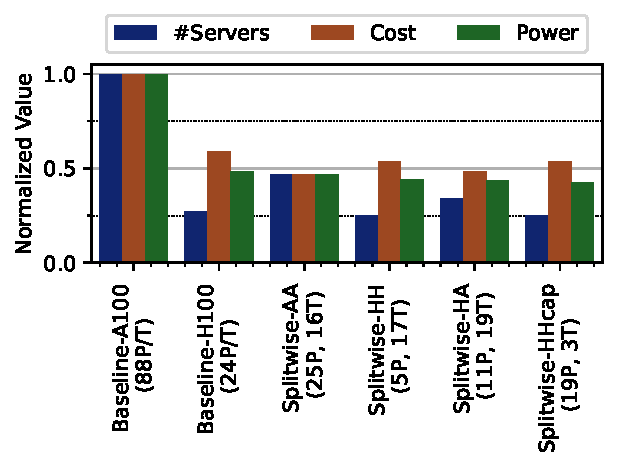
\includegraphics[width=0.48\columnwidth]{figures/eval/isothroughput_conv_cost_bloom-176b}
        \label{fig:isotputcost}
    }
    \caption{Summary of iso-throughput cluster designs.}
    \label{fig:isotput}
\end{figure}



\subsection{Other cluster optimizations}
We have described \emph{iso-power throughput-optimized clusters} in detail.
For the rest of the cluster optimization evaluation, we only discuss the summary plots.

\myparagraph{Iso-cost throughput-optimized}
\Cref{fig:isocosttput} shows the summary plot for iso-cost clusters, with their space, throughput, and power requirements.
We find that Splitwise-AA provides the best throughput for the same cost, namely 1.4$\times$ more throughput than Baseline-H100, running at 25\% more power, and 2$\times$ the space.
This is an interesting operational point for most customers who may not care about power and space, instead preferring the 40\% higher throughput using older, more easily available GPUs.
In contrast, the preferable choice for the CSP is less clear.

\myparagraph{Iso-throughput power-optimized}
\Cref{fig:isotputpower} shows cluster designs that yield same throughput at the least power.
Splitwise-HHcap can achieve the same throughput as Baseline-H100 at 25\% lower power at the same cost and space.
This can be a clear win for the CSPs.

\myparagraph{Iso-throughput cost-optimized}
\Cref{fig:isotputcost} shows the cost-optimized versions of the iso-throughput design.
Note that there are no changes to any of the homogeneous designs between \Cref{fig:isotputpower,fig:isotputcost}.
This is because the prompt and token machines have the same cost and power.
However, Splitwise-HA and Splitwise-HHcap arrive at slightly different results with the cost and power optimizations.
\Cref{fig:isotputcost} shows that with Splitwise-AA, customers can achieve the same throughput as Baseline-H100 at 25\% lower cost.


\subsection{Impact of workload changes}
\label{subsec:exp-workload-changes}
So far, we have tested a trace and a model on clusters optimized for a specific workload pattern and model.
To test the Splitwise' robustness, we now run conversation trace on a cluster meant for coding service, and Llama-70B on a cluster meant for BLOOM-176B.
\Cref{fig:switcharoo} shows these results for iso-power throughput-optimized clusters.

\myparagraph{Changing workload trace}
Compared to \Cref{fig:isopowerfullconv}, we find that in \Cref{fig:convoncode}, the Baseline clusters are similarly sized and incur no throughput or latency impact.
Splitwise-AA and Splitwise-HH with the mixed pool morph well to meet the requirements of the new workload, and they see no throughput or latency impact.
Since Splitwise-HA and Splitwise-HHcap have different types of machines in the prompt and token pools, they experience a throughput setback of 7\% from the respective cluster optimized designs for conversation trace. Note that all the Splitwise designs still perform much better than any of the Baseline designs. 

\myparagraph{Changing model}
\Cref{fig:llamaonbloom} shows that Llama-70B can support much higher throughput in the same cluster design than BLOOM-176B, given its fewer parameters (\Cref{tab:models}).
All the Splitwise designs out-perform both the Baseline designs at higher load.
Furthermore, Splitwise-HH and Splitwise-HHcap consistently achieve the best latency, even as the load increases.

\myparagraph{Summary}
Based on these two experiments, we conclude that Splitwise can morph according to the requirements of the workload using its smart scheduling, and it is robust to changes in the LLMs, request load, and token distributions.

\begin{figure}
    \centering
     \subfloat[Conversation trace running on a cluster designed for coding.]{
        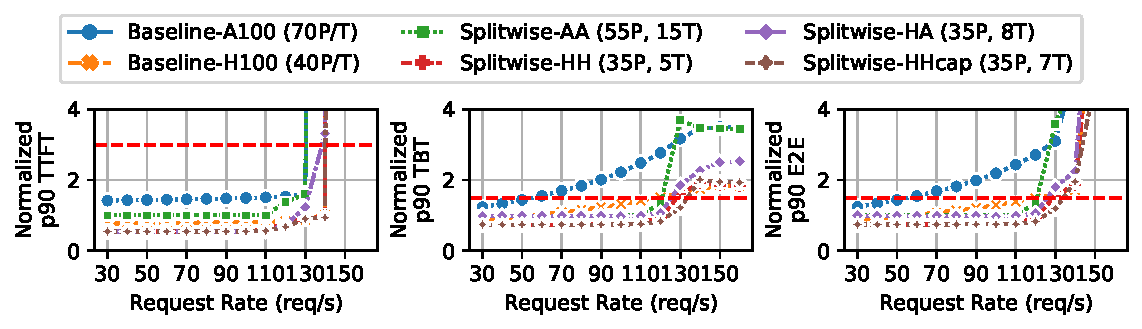
\includegraphics[width=1.0\columnwidth]{figures/eval/isopower_code_for_conv_bloom-176b_p90}
        \label{fig:convoncode}
    }
    \vspace{0pt}
    \subfloat[Llama-70B, on a cluster designed for BLOOM-176B.]{
        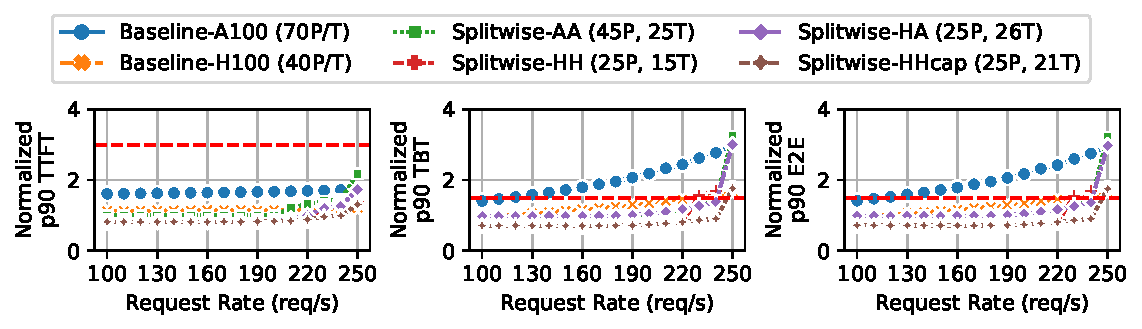
\includegraphics[width=1.0\columnwidth]{figures/eval/isopower_conv_llama2-70b_p90}
        \label{fig:llamaonbloom}
    }
    \caption{Latency impact of running a workload on a cluster designed for another workload. Dashed red lines indicate SLO.}
    \label{fig:switcharoo}
    %\vspace*{-0.5cm}
\end{figure}


\subsection{Cluster design for batch job}
We design various clusters with Splitwise under strict latency SLOs, even when we are optimizing for throughput.
This is unnecessary for batch jobs, which can be stressed to high load for a high token generation throughput.
We find that upon stressing our iso-power throughput-optimized clusters, Baseline-A100 and Splitwise-AA have the best throughput per cost at 0.89 RPS/\$.
At high load, Splitwise devolves into the iso-count Baseline, since it starts mixed batching with all the machines in the mixed pool.
The same holds true for Splitwise-HH and Baseline-H100, which achieve 0.75 RPS/\$.
